\documentclass{standalone}
%
\usepackage{tikz}
\usetikzlibrary{backgrounds,arrows.meta,shapes.callouts}
\usepackage{xcolor}
%
\definecolor{space}{HTML}{1F2C4E}
\definecolor{earth}{HTML}{0089FA}
\definecolor{dida}{HTML}{FFDE00}
\definecolor{title}{HTML}{FBA706}
\definecolor{galaxy}{HTML}{4278A4}
%
\usepackage{fontspec}
\setmainfont{Open Dyslexic}
%
\title{Esopianeti}
\begin{document}
	\tikzset{
		partial ellipse/.style args = {#1:#2:#3}{insert path={+ (#1:#3) arc (#1:#2:#3)}},
		notice/.style  = { draw, ellipse callout, callout relative pointer={#1} },
	}
	\begin{tikzpicture}[background rectangle/.style={fill=white},show background rectangle,>={[inset=0,angle'=27]Stealth}]
		%title
		\draw [black,ultra thick,fill=title] (0,9.8) rectangle (30,16.8);
		\node at (15,14.8) {\textcolor{black}{\fontsize{75}{76}\selectfont Esopianeti fantastici}};
		\node at (15,11.8) {\textcolor{black}{\fontsize{75}{76}\selectfont e dove trovarli}};
		%
		\begin{scope}[shift={(0,1.5)}]
			\draw [ultra thick, fill=space] (1,0) rectangle (29,-2);
		\end{scope}
		%
		\begin{scope}[shift={(0,5)}]
			\draw [ultra thick, fill=earth] (20.5,4) rectangle (25.5,-4);
			\node at (23,0) {
\includegraphics[width=5cm]{carl_sagan}};
			\node (example-textwidth-2) [notice={(3,0.5)}, ultra thick, right, align=center, text width=12cm, color=black, fill=white, font=\fontsize{23pt}{24pt}\selectfont] at (1,-1) {Gli scrittori di fantascienza hanno ideato pianeti fantastici che ruotano intorno a stelle lontane.};
		\end{scope}
		%
		\begin{scope}[shift={(0,-3)}]
			\draw [ultra thick, fill=earth] (5.5,4) rectangle (10.5,-4);
			\node at (8,0) {
\includegraphics[width=5cm]{carl_sagan}};
			\node (example-textwidth-2) [notice={(-3,0.5)}, ultra thick, right, align=center, text width=12cm, color=black, fill=white, font=\fontsize{23pt}{24pt}\selectfont] at (12,-1) {E alcuni degli esopianeti scoperti in questi anni gli assomigliano! Andiamo a scoprirne qualcuno!};
		\end{scope}
		% Tatooine
		\begin{scope}[shift={(0,-13)}]
			\draw [fill=black] (1,3) rectangle (28,-14);
			%
			\draw [fill=earth!50!white, thick] (14.5,4.5) rectangle (26.5,-15);
			%
			\draw [fill=galaxy, ultra thick] (14,3.5) rectangle (27,-3);
			\draw [fill=dida, ultra thick] (2,4) rectangle (27.5,1);
			%
			\draw [fill=title, thick] (14,-5.8) rectangle (27,-6.7);
			\draw [fill=title, thick] (14,-12.1) rectangle (27,-13);
			%
			\node (example-textwidth-2) [right, align=left, text width=25cm, color=black, font=\fontsize{23pt}{24pt}\selectfont] at (2.5,2.5) {Il più noto di tutti è Tatooine, comparso in \emph{Guerre stellari}. Ruota intorno a una stella doppia.};
			\node (example-textwidth-2) [right, align=left, text width=12cm, color=black, font=\fontsize{23pt}{24pt}\selectfont] at (15,-1) {Proprio come Kepler-1647 b, che però è un pianeta gassoso.};
			\node at (8,-5) {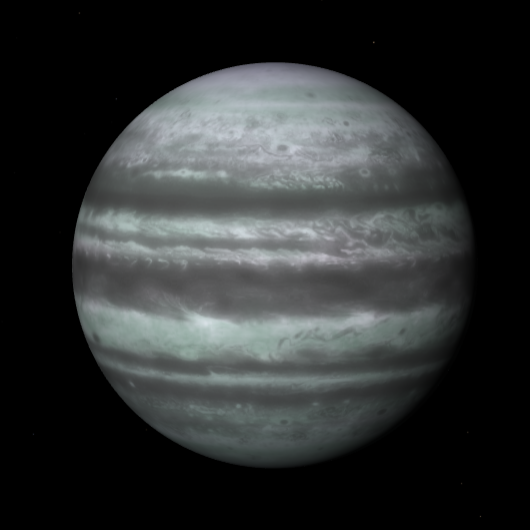
\includegraphics[width=9cm]{kepler1647b}};
			\node (example-textwidth-2) [right, align=center, text width=12cm, color=white, font=\fontsize{18pt}{19pt}\selectfont] at (2,-9.8) {Rappresentazione ipotetica realizzata dalla NASA};
			%
			\node (example-textwidth-2) [right, align=left, text width=12cm, color=black, font=\fontsize{18pt}{19pt}\selectfont] at (15,-4.2) {\textbf{Scoperto da}: Kepler Space Observatory il 13 giugno 2016\\\textbf{Metodo}: Transito};
			\node (example-textwidth-2) [right, align=left, text width=12cm, color=black, font=\fontsize{18pt}{19pt}\selectfont] at (15,-6.2) {\textbf{Caratteristiche orbitali}};
			\node (example-textwidth-2) [right, align=left, text width=10cm, color=black, font=\fontsize{18pt}{19pt}\selectfont] at (15,-9.5) {\textbf{Semiasse maggiore}: 2.7205 ± 0.007 AU\\\textbf{Eccentricità}: 0.0581\\\textbf{Periodo orbitale}: 1107.6±0.023 giorni\\\textbf{Inclinazione}: -90.1\\\textbf{Stella}: Kepler-1647};
			\node (example-textwidth-2) [right, align=left, text width=12cm, color=black, font=\fontsize{18pt}{19pt}\selectfont] at (15,-12.5) {\textbf{Caratteristiche fisiche}};
			\node (example-textwidth-2) [right, align=left, text width=12cm, color=black, font=\fontsize{18pt}{19pt}\selectfont] at (15,-14) {\textbf{Raggio medio}: 1.06±0.0123 RG\\\textbf{Massa}: 1.52±0.65 MG};
		\end{scope}
		% Gallia
		\begin{scope}[shift={(0,-34)}]
			\draw [fill=black] (1,3) rectangle (28,-21.5);
			%
			\draw [fill=earth!50!white, thick] (14.5,4.5) rectangle (26.5,-23.5);
			%
			\draw [fill=dida, ultra thick] (2,4) rectangle (27.5,1);
			%
			\node (example-textwidth-2) [right, align=left, text width=25cm, color=black, font=\fontsize{23pt}{24pt}\selectfont] at (2.5,2.5) {E poi c'è Gallia, una cometa grande come un asteroide destritta da \textbf{Jules Verne} in uno dei suoi romanzi \emph{astrofantastici}.};
			\draw [fill=galaxy, ultra thick] (14,-7.5) rectangle (27,-9.5);
			\node (example-textwidth-2) [right, align=left, text width=12cm, color=black, font=\fontsize{23pt}{24pt}\selectfont] at (14.8,-8.5) {Solo che anche HD 209458b è un pianeta gassoso.};
			\node at (8,-13) {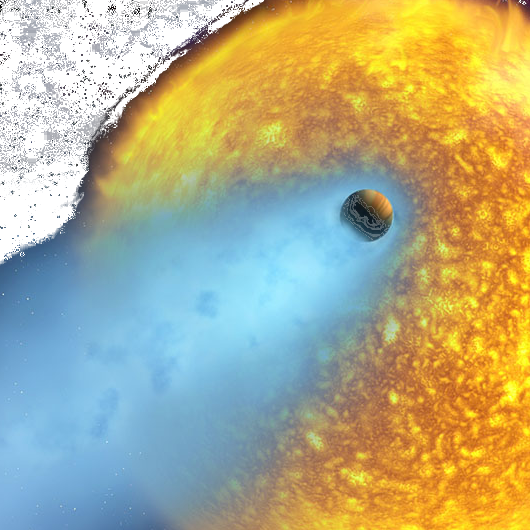
\includegraphics[width=9cm]{hd209458b}};
			\node (example-textwidth-2) [right, align=center, text width=12cm, color=white, font=\fontsize{18pt}{19pt}\selectfont] at (2,-19) {Rappresentazione ipotetica realizzata dalla NASA};
			%
			\node (example-textwidth-2) [right, align=left, text width=10cm, color=black, font=\fontsize{18pt}{19pt}\selectfont] at (15,-11) {\textbf{Scoperto da}: \textbf{D. Charbonneau} \emph{et al.} il 9 settembre 1999\\\textbf{Metodo}: Velocità radiale};
			\draw [fill=title, thick] (14,-12.6) rectangle (27,-13.5);
			\node (example-textwidth-2) [right, align=left, text width=12cm, color=black, font=\fontsize{18pt}{19pt}\selectfont] at (15,-13) {\textbf{Caratteristiche orbitali}};
			\node (example-textwidth-2) [right, align=left, text width=10cm, color=black, font=\fontsize{18pt}{19pt}\selectfont] at (15,-16.5) {\textbf{Semiasse maggiore}: 0.04747 AU\\\textbf{Eccentricità}: 0.014±0.009\\\textbf{Periodo orbitale}: 3.52474541 ± 0.00000025 giorni e 84.5938898 ore\\\textbf{Inclinazione}: 86.1 ± 0.1\\\textbf{Stella}: HD 209458};
			\draw [fill=title, thick] (14,-19.6) rectangle (27,-20.5);
			\node (example-textwidth-2) [right, align=left, text width=12cm, color=black, font=\fontsize{18pt}{19pt}\selectfont] at (15,-20) {\textbf{Caratteristiche fisiche}};
			\node (example-textwidth-2) [right, align=left, text width=12cm, color=black, font=\fontsize{18pt}{19pt}\selectfont] at (15,-22) {\textbf{Raggio medio}: 1.06±0.0123 RG\\\textbf{Massa}: 1.52±0.65 MG\\\textbf{Gravità}: 0.96 g};
			%
			\node at (8,-3) {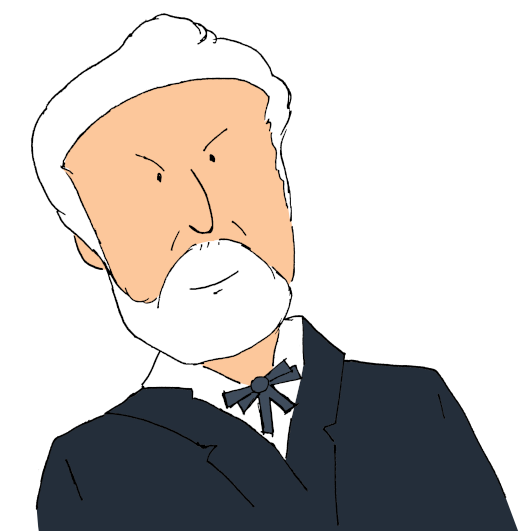
\includegraphics[width=8cm]{verne}};
			\node (example-textwidth-2) [notice={(-3,0.5)}, ultra thick, right, align=center, text width=12cm, color=black, fill=white, font=\fontsize{23pt}{24pt}\selectfont] at (12,-3) {Non sapevamo che comete così grandi non potevano esistere, però è bello sapere che è stato scoperto un pianeta con la coda!};
		\end{scope}
		% Apokolips
		\begin{scope}[shift={(0,-63)}]
			\draw [fill=black] (1,3) rectangle (28,-12);
			%
			\draw [fill=earth!50!white, thick] (14.5,4.5) rectangle (26.5,-13);
			%
			\draw [fill=dida, ultra thick] (2,4) rectangle (27.5,0.8);
			%
			\node (example-textwidth-2) [right, align=left, text width=25cm, color=black, font=\fontsize{23pt}{24pt}\selectfont] at (2.5,2.5) {Apokolips, ideato dal fumettista \textbf{Jack Kirby}, è un pianeta la cui superficie è letteralmente infernale. Proprio come 55 Cancri-e.};
			\node at (8,-5) {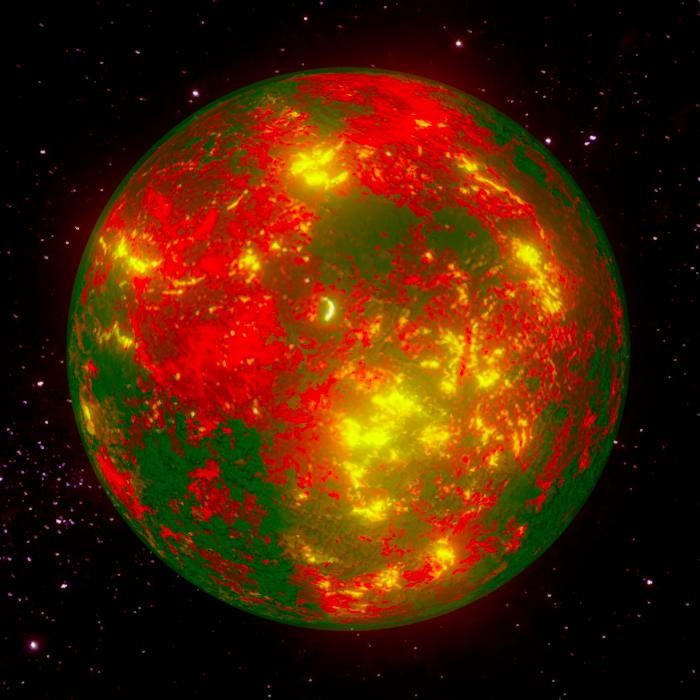
\includegraphics[width=9cm]{55cancrie}};
			\node (example-textwidth-2) [right, align=center, text width=12cm, color=white, font=\fontsize{18pt}{19pt}\selectfont] at (2,-10) {Rappresentazione ipotetica realizzata dall'Osservatorio Astronomico di Palermo};
			%
			\node (example-textwidth-2) [right, align=left, text width=10cm, color=black, font=\fontsize{18pt}{19pt}\selectfont] at (15,-1.2) {\textbf{Scoperto da}: \textbf{McArthur} \emph{et al.} il 30 agosto 2004\\\textbf{Metodo}: Velocità radiale};
			%
			\draw [fill=title, thick] (14,-2.8) rectangle (27,-3.7);
			\node (example-textwidth-2) [right, align=left, text width=12cm, color=black, font=\fontsize{18pt}{19pt}\selectfont] at (15,-3.2) {\textbf{Caratteristiche orbitali}};
			\node (example-textwidth-2) [right, align=left, text width=10cm, color=black, font=\fontsize{18pt}{19pt}\selectfont] at (15,-6.5) {\textbf{Semiasse maggiore}: 0.01544 ± 0.00005 AU\\\textbf{Eccentricità}: 0.05 ± 0.03\\\textbf{Periodo orbitale}: 0.7365474 ± 0.0000014 giorni e 17.677 ore\\\textbf{Inclinazione}: 83.59\\\textbf{Stella}: 55 Cancri A};
			%
			\draw [fill=title, thick] (14,-9.1) rectangle (27,-10);
			\node (example-textwidth-2) [right, align=left, text width=12cm, color=black, font=\fontsize{18pt}{19pt}\selectfont] at (15,-9.5) {\textbf{Caratteristiche fisiche}};
			\node (example-textwidth-2) [right, align=left, text width=12cm, color=black, font=\fontsize{18pt}{19pt}\selectfont] at (15,-11.5) {\textbf{Raggio medio}: 1.06±0.0123 RT\\\textbf{Massa}: 1.52±0.65 MT\\\textbf{Gravità}: 2.273 g};
		\end{scope}
		% Vulcano
		\begin{scope}[shift={(0,-82)}]
			\draw [fill=black] (1,3) rectangle (28,-26);
			%
			\draw [fill=earth!50!white, thick] (14.5,5) rectangle (26.5,-27);
			%
			\draw [fill=dida, ultra thick] (2,4.5) rectangle (27.5,0.5);
			%
			\node at (8,-6.5) {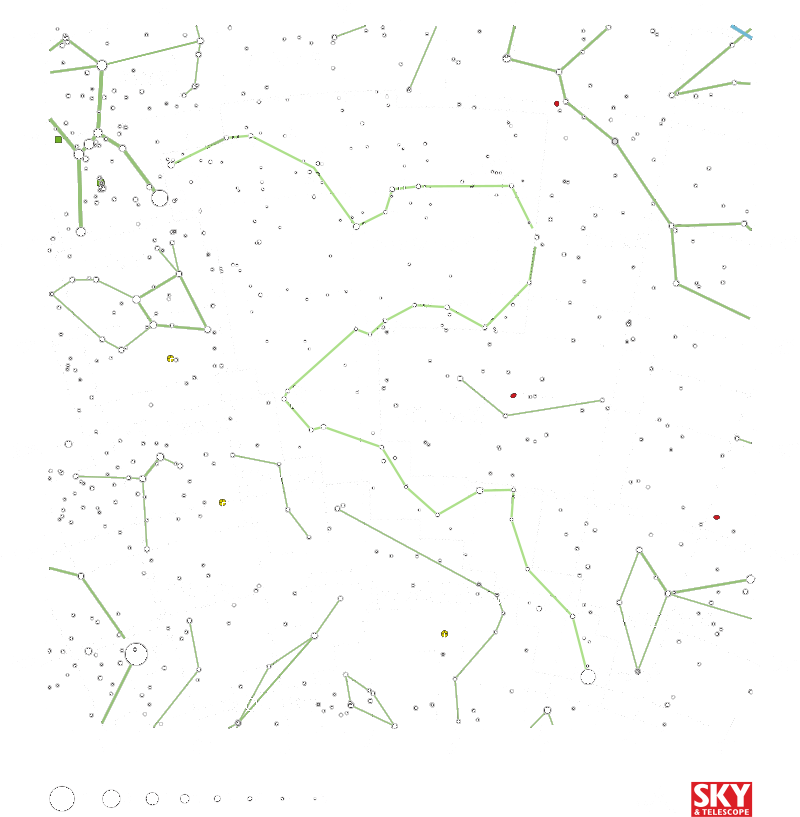
\includegraphics[width=12cm]{eridano}};
			%
			\node (example-textwidth-2) [right, align=left, text width=25cm, color=black, font=\fontsize{23pt}{24pt}\selectfont] at (2.5,2.5) {Facciamo un balzo nella costellazione di Eridano. Qui si trova una stella tripla, 40 Eridani. E una delle stelle del sistema, 40 Eridani A, nella cui zona abitabile è stata trovata una \emph{Super Terra}!};
			\node at (8,-18) {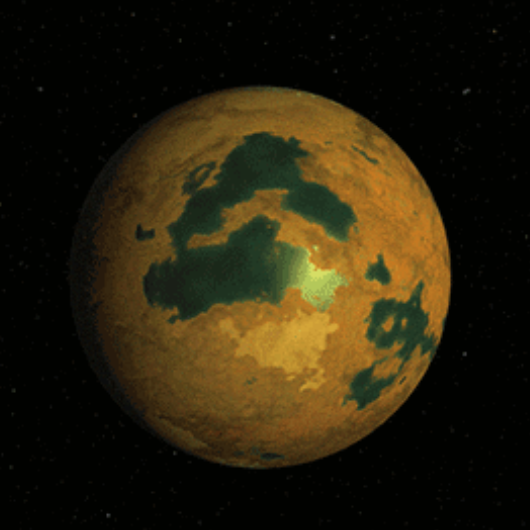
\includegraphics[width=9cm]{vulcano}};
			\node (example-textwidth-2) [right, align=center, text width=12cm, color=white, font=\fontsize{18pt}{19pt}\selectfont] at (2,-24) {Rappresentazione immaginaria di Vulcano realizzata dalla NASA};
			%
			\node (example-textwidth-2) [right, align=left, text width=10cm, color=black, font=\fontsize{18pt}{19pt}\selectfont] at (15,-1.2) {\textbf{Scoperto da}: \textbf{Bo Ma} \emph{et al.} nel 2018\\\textbf{Metodo}: Velocità radiale};
			%
			\draw [fill=title, thick] (14,-2.6) rectangle (27,-3.5);
			\node (example-textwidth-2) [right, align=left, text width=12cm, color=black, font=\fontsize{18pt}{19pt}\selectfont] at (15,-3) {\textbf{Caratteristiche orbitali}};
			\node (example-textwidth-2) [right, align=left, text width=10cm, color=black, font=\fontsize{18pt}{19pt}\selectfont] at (15,-6) {\textbf{Semiasse maggiore}: 0.22446±0.00004 AU\\\textbf{Eccentricità}: 0.04\\\textbf{Periodo orbitale}: 42.378 ± 0.01 giorni\\\textbf{Stella}: 40 Eridani A};
			%
			\draw [fill=title, thick] (14,-8.3) rectangle (27,-9.2);
			\node (example-textwidth-2) [right, align=left, text width=12cm, color=black, font=\fontsize{18pt}{19pt}\selectfont] at (15,-8.7) {\textbf{Caratteristiche fisiche}};
			\node (example-textwidth-2) [right, align=left, text width=12cm, color=black, font=\fontsize{18pt}{19pt}\selectfont] at (15,-10) {\textbf{Massa}: 8.47 ± 0.47 MT};
			%
			\draw [fill=dida, ultra thick] (14,-14.5) rectangle (27,-21.5);
			\node (example-textwidth-2) [right, align=left, text width=12cm, color=black, font=\fontsize{23pt}{24pt}\selectfont] at (14.8,-18) {La curiosità è che da qualche parte nel sistema triplo di 40 Eridani ruoterebbe, secondo gli autori di \emph{Star Trek}, Vulcano, il pianeta d'origine del mitico Spock.};
		\end{scope}
		% kepler
		\begin{scope}[shift={(0,-112)}]
			\draw [fill=space,thick] (1,2) rectangle (29,-2);
			%
			\node (example-textwidth-2) [right, align=left, text width=25cm, color=white, font=\fontsize{23pt}{24pt}\selectfont] at (2.5,0) {AU: Unità astronomica. La distanza Terra-Sole\\MG, RG: Massa e raggio di Giove\\MT, RT: Massa e raggio della Terra};
			\draw [fill=dida, ultra thick] (1.2,1.5) rectangle (5.8,2.5);
			\node (example-textwidth-2) [right, align=left, text width=25cm, color=black, font=\fontsize{23pt}{24pt}\selectfont] at (1.5,2) {Legenda:};
		\end{scope}
		%
		\begin{scope}[shift={(0,-115)}]
			\node at (27,0) () {
\includegraphics[width=3.7cm]{licenza}};
			\node (example-textwidth-2) [right, align=left, text width=14cm, color=black, font=\fontsize{14pt}{15pt}\selectfont] at (11,-0.1) {Testo e illustrazioni (laddove diversamente indicato): @ulaulaman - Gianluigi Filippelli};
		\end{scope}
	\end{tikzpicture}
\end{document}
